\section{Analyse af datasæt}

\paragraph{8.}
Vi indlæser vores datasæt i R ved følgende kommando:

\begin{figure}[H]
\label{fig:anal0}
\begin{center}
\begin{verbatim}
avit <- read.table("avit.txt", header=TRUE)
\end{verbatim}
\caption{}
\end{center}
\end{figure}

\paragraph{9.}
Der laves først en variabel, avitM, hvori vi ligger udtaget af 
mændenes A-vitaminindtag på:

\begin{figure}[H]
\label{fig:anal1}
\begin{center}
\begin{verbatim}
> avitM <- subset(avit, sex==1)$avit
\end{verbatim}
\caption{}
\end{center}
\end{figure}

Herefter bestemmes antallet:

\begin{figure}[H]
\label{fig:anal2}
\begin{center}
\begin{verbatim}
> length(avitM)
[]  1079
\end{verbatim}
\caption{}
\end{center}
\end{figure}

Der laves nu endnu en variabel, der indeholder logaritmen til 
værdierne i avitM:

\begin{figure}[H]
\label{fig:anal3}
\begin{center}
\begin{verbatim}
> logavitM <- log(avitM)
\end{verbatim}
\caption{}
\end{center}
\end{figure}

\paragraph{10.}
Vi indtegner nu histogrammer henholdsvis for avitM og logavitM:

\begin{figure}[H]
\label{fig:anal4}
\begin{center}
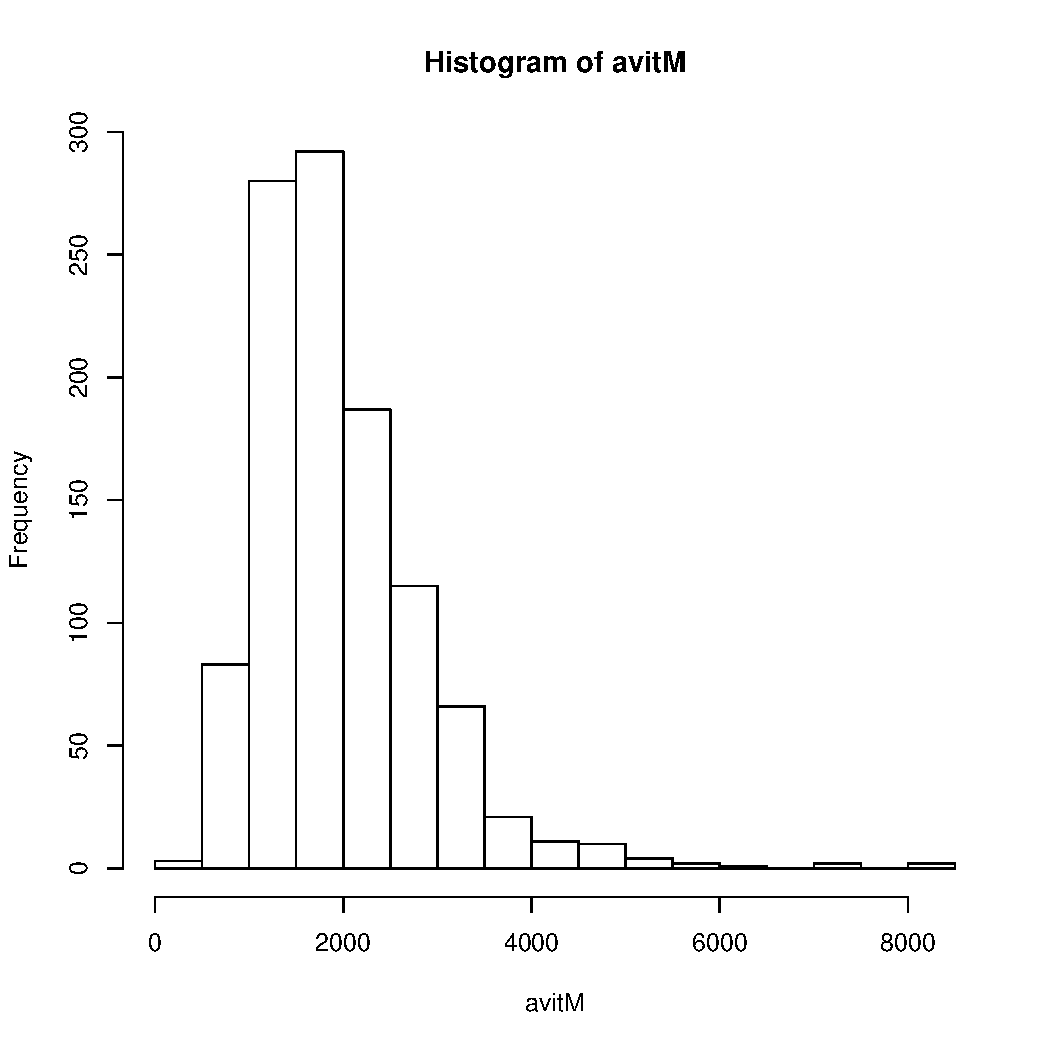
\includegraphics[width=10cm]{graphs/analyse_1.pdf}
\caption{Histogram for avitM}
\end{center}
\end{figure}

\begin{figure}[H]
\label{fig:anal5}
\begin{center}
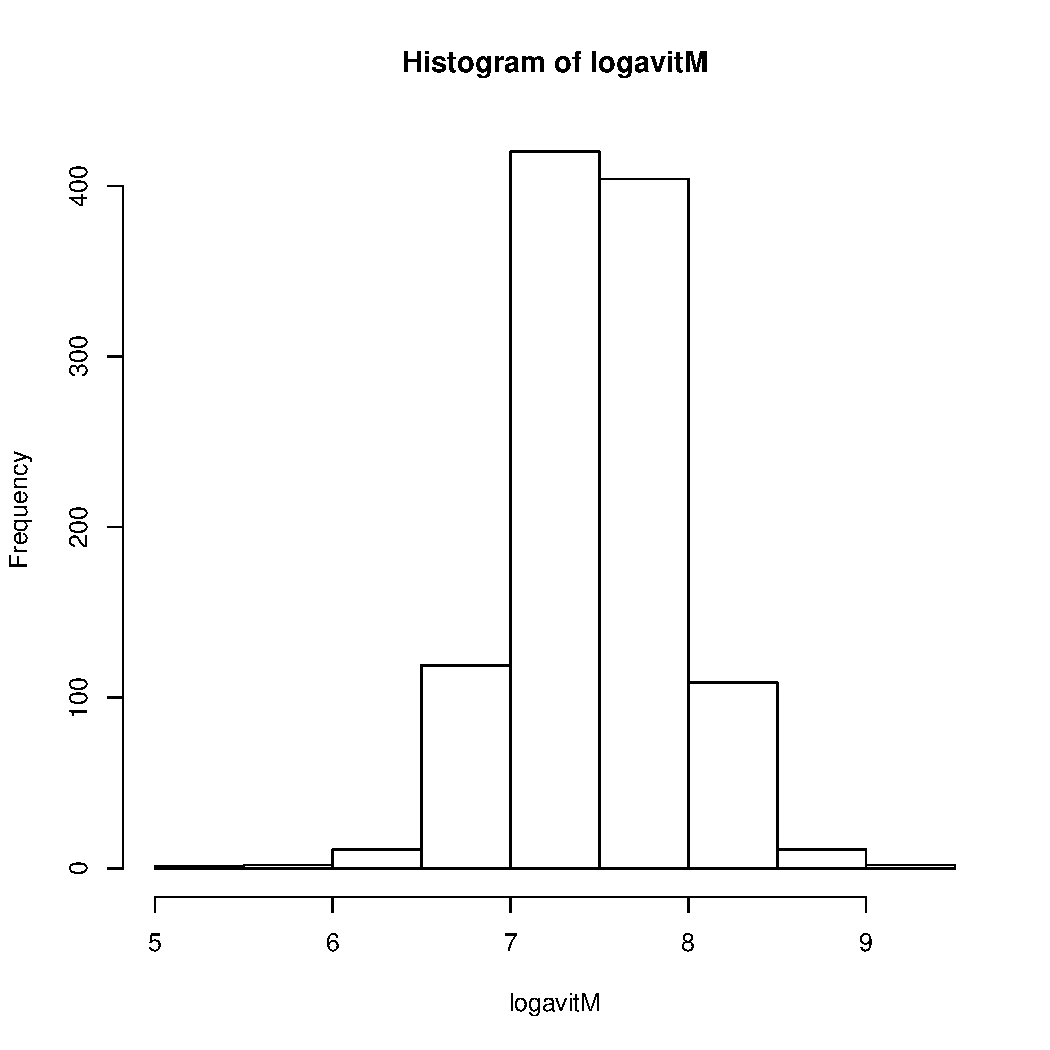
\includegraphics[width=10cm]{graphs/analyse_3.pdf}
\caption{Histogram for logavitM}
\end{center}
\end{figure}


Som vi kan se ser grafen for logaritmen til indtaget af A-vitamin mere
normalfordelt ud end grafen for de rene data.

Nedenfor følger QQ-plots for avitM og logavitM:

\begin{figure}[H]
\label{fig:anal6}
\begin{center}
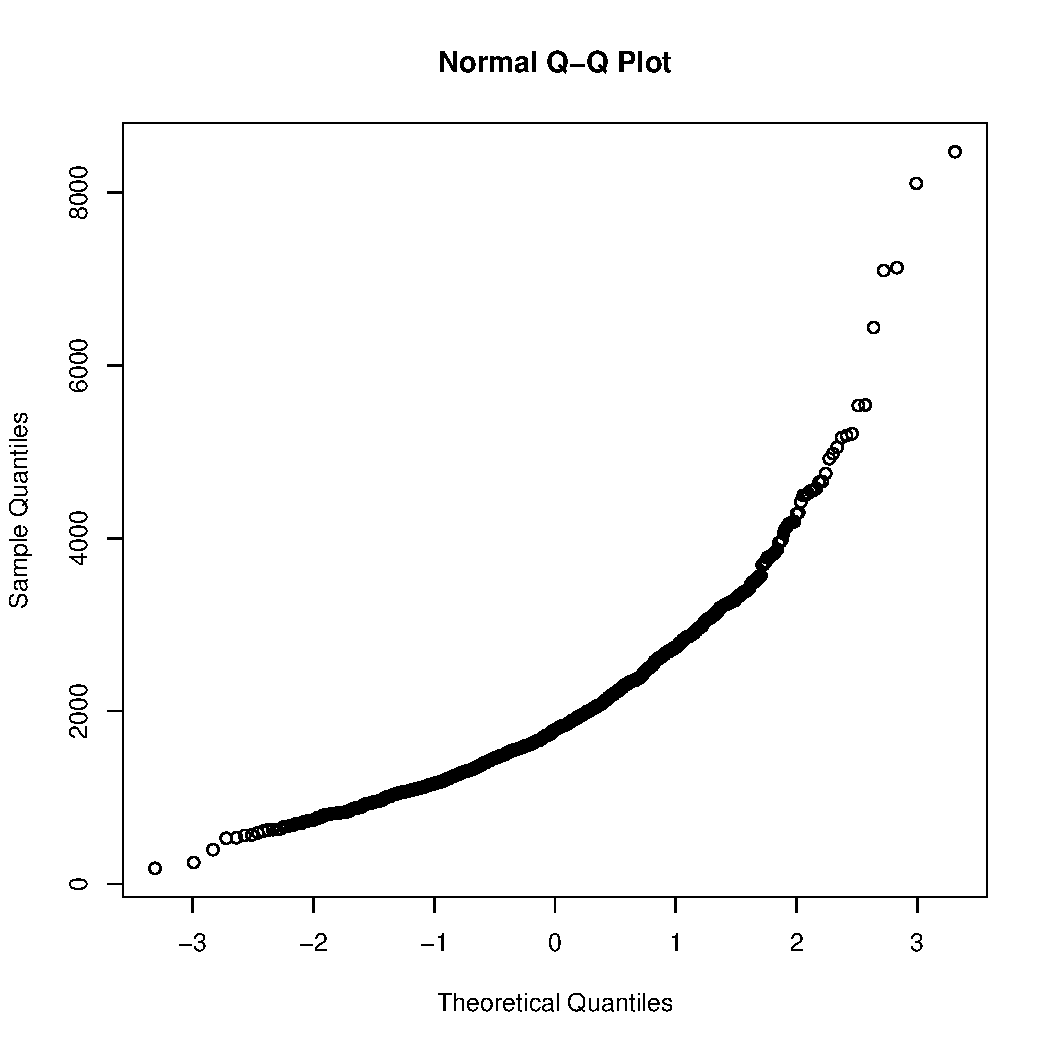
\includegraphics[width=10cm]{graphs/analyse_2.pdf}
\caption{QQ-plot for avitM}
\end{center}
\end{figure}

\begin{figure}[H]
\label{fig:anal7}
\begin{center}
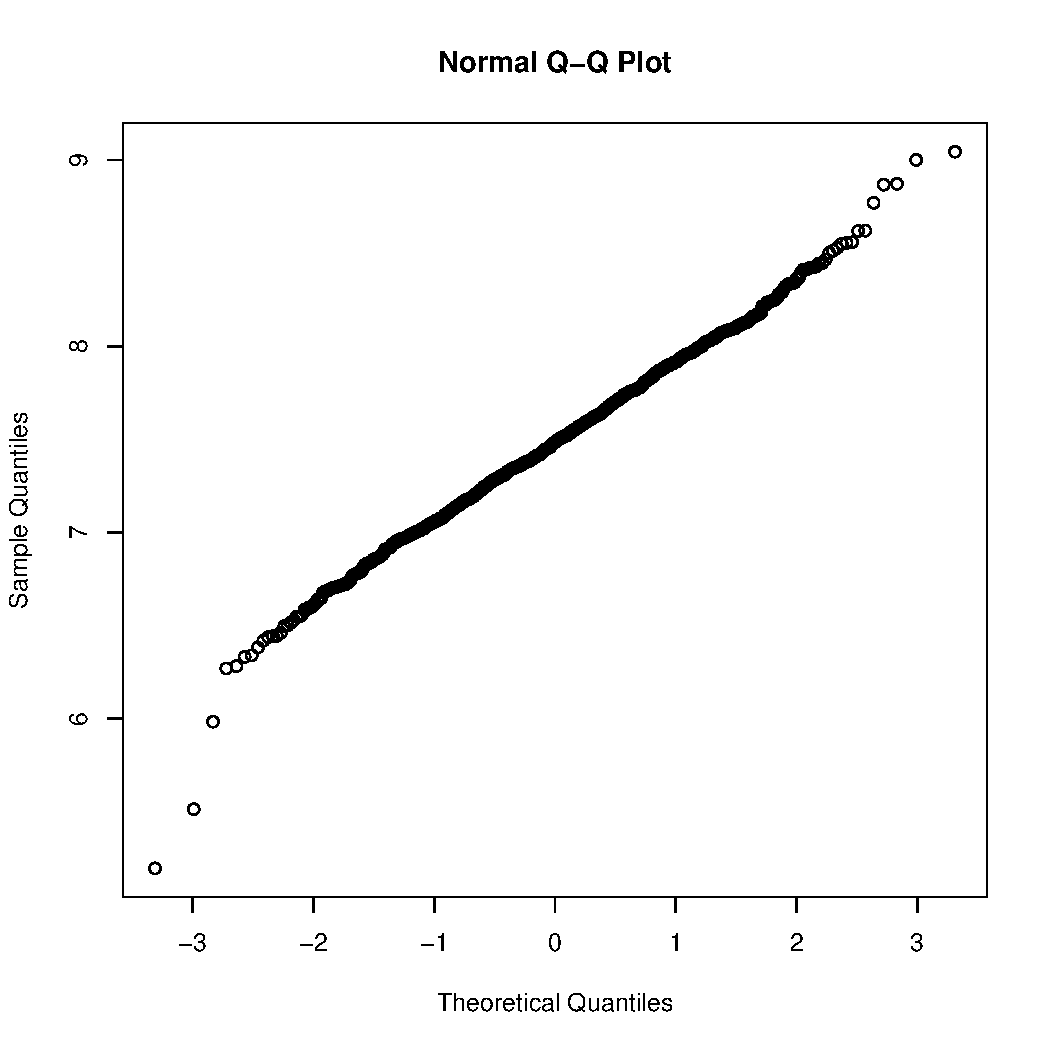
\includegraphics[width=10cm]{graphs/analyse_4.pdf}
\caption{Histogram for avitM}
\end{center}
\end{figure}

Vi ser her tydeligt, at grafen for de logaritmiske data er en meget
bedre approksimation til en normalfordeling.

\paragraph{11.} 
Gennemsnit for logavitM beregnes:

\begin{figure}[H]
\label{fig:anal8}
\begin{center}
\begin{verbatim}
> mean(logavitM)
[]  7.484993
\end{verbatim}
\caption{}
\end{center}
\end{figure}

Stikprøvevarians for logavitM beregnes:

\begin{figure}[H]
\label{fig:anal9}
\begin{center}
\begin{verbatim}
> var(logavitM)
[]  0.1916541
\end{verbatim}
\caption{}
\end{center}
\end{figure}

Stikprøvespredning for logavitM beregnes:

\begin{figure}[H]
\label{fig:anal10}
\begin{center}
\begin{verbatim}
> sd(logavitM)
[]  0.4377832
\end{verbatim}
\caption{}
\end{center}
\end{figure}

\paragraph{12.}
Histogrammet for logavitM indtegnes denne gang med tætheden for 
normalfordelingen med middelværdi og varians som fundet tidligere:

\begin{figure}[H]
\label{fig:anal11}
\begin{center}
\begin{verbatim}
> hist(logavitM, prop=T, nclass=25)
> f = function(x) dnorm(x, mean(logavitM), sd(logavitM))
> plot(f, 0, 9, add=T)
\end{verbatim}
\caption{}
\end{center}
\end{figure}

\begin{figure}[H]
\label{fig:anal12}
\begin{center}
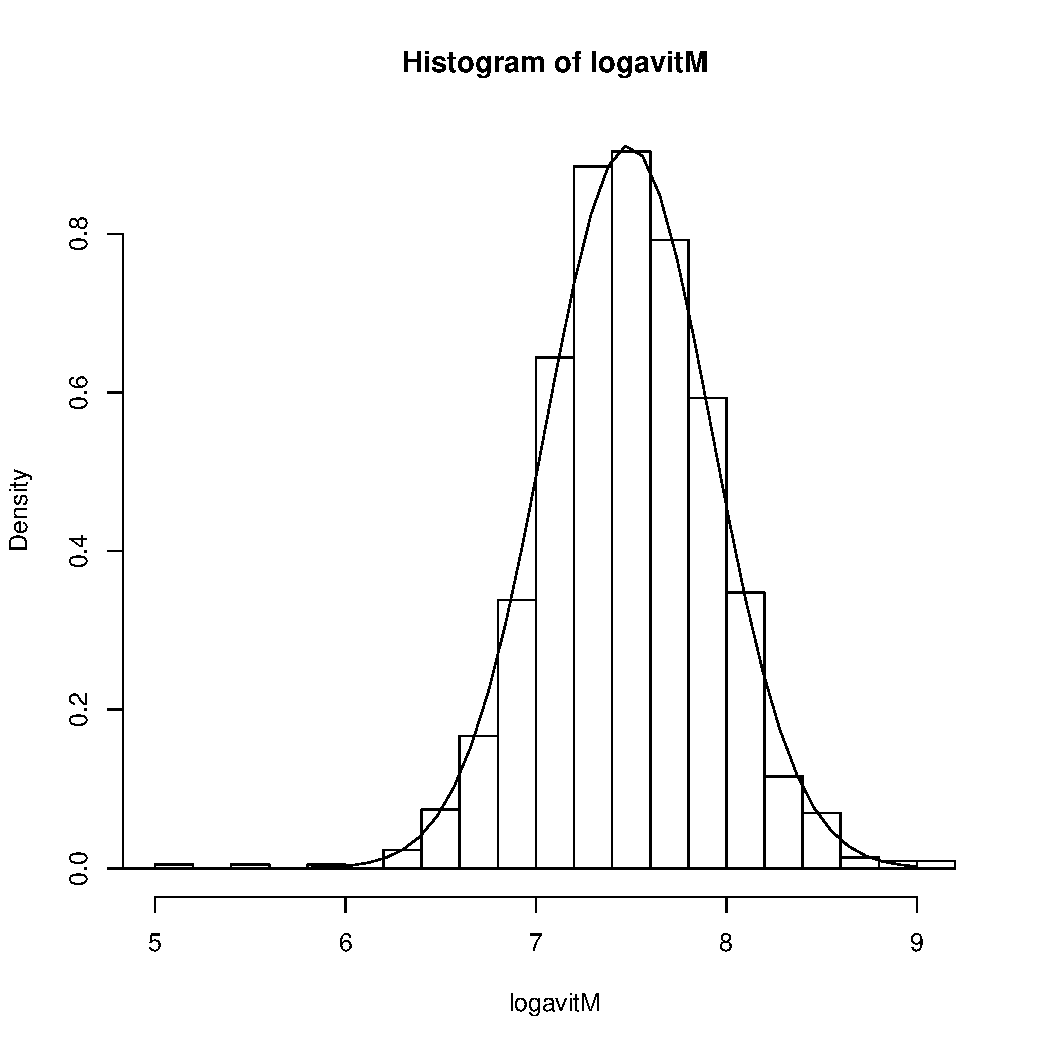
\includegraphics[width=10cm]{graphs/analyse_5.pdf}
\caption{Histogram for logavitM med normalfordelingen indtegnet}
\end{center}
\end{figure}

Histogrammet for avitM indtegnes denne gang sammen med tætheden for 
den tilhørende logaritmiske normalfordeling:

\begin{figure}[H]
\label{fig:anal13}
\begin{center}
\begin{verbatim}
> lnorm = function(y, mu, sigma) 1/(y*sqrt(2*pi*sigma^2)) * 
> exp(-((log(y) - mu)^2) / (2*sigma^2))
> hist(avitM, prop=T, nclass=25)
> g = function(x) lnorm(x, mean(logavitM), sd(logavitM))
> plot(g, 0, 8000, add=T)
\end{verbatim}
\caption{}
\end{center}
\end{figure}

\begin{figure}[H]
\label{fig:anal14}
\begin{center}
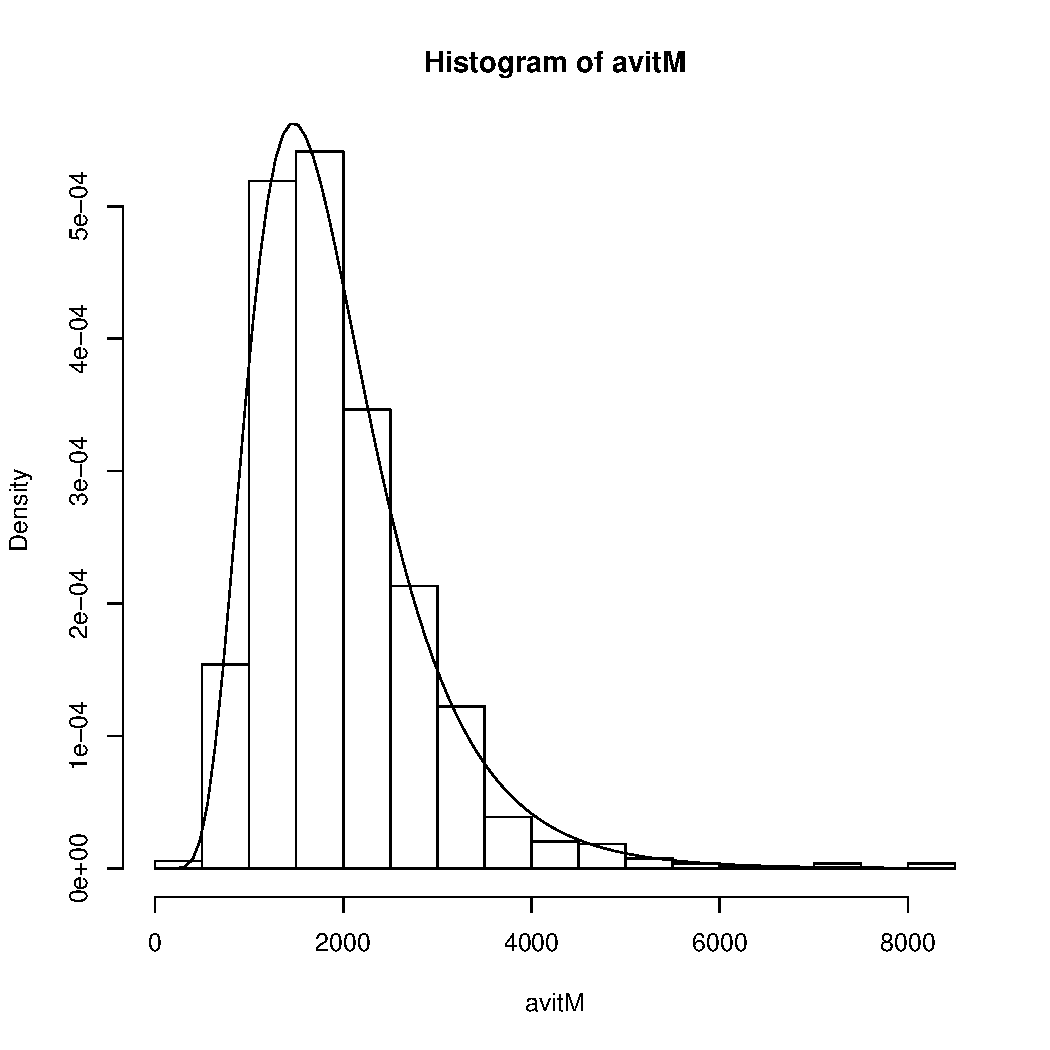
\includegraphics[width=10cm]{graphs/analyse_6.pdf}
\caption{Histogrammet for avitM med den tilhørende logaritmiske normalfordeling}
\end{center}
\end{figure}

Som vi kan se passer den tætheden for den logaritmiske normalfordeling
godt på histogrammet over indtaget af A-vitaminer. Ligeledes passer
passer tætheden af normalfordelingen med den fundne middelværdi og
varians også godt med histogrammet for logavitM.

\paragraph{13.}
Den statistike model er givet ved udfaldsrummet $E=[0; \infty)$ samt
  familien

\begin{equation*}
  \mathcal{P} =\{ N^n_{\mu,\sigma^2} : (\mu, \sigma^2) \in \mathbb{R}
  \times (0, \infty) \}
\end{equation*}

af fordelinger på $\mathbb{R}^2$ hvor $N^n_{\mu, \sigma^2}$ har tæthed

\begin{equation*}
  f_{\mu, \sigma^2}(y) = \frac{1}{y \sqrt{2\pi\sigma^2}} exp ( -
  \frac{(log y - \mu)^2}{2\sigma^2} ), y>0
\end{equation*}

For de $1079$ $y_1, \ldots, y_{1079}$ af logaritmen af nogle mænds
indtag af a-vitaminer har vi fået at

\begin{equation*}
  \bar{y} = 7,485, \quad ssd = \Sigma^{1079}_{i=1}(y_i - \bar{y})^2 =
  206,6031
\end{equation*}

Estimaterne er altså

\begin{equation*}
  \hat{\mu} = 7,485, \quad s^2 = \frac{206,6031}{1079-1} = 0,1917, \quad
  s = 0,4378
\end{equation*}

Den estimerede fordeling for $\hat{\mu}$ er $N(7,485;
\frac{0,1917}{1079} = 1,7762 * 10^{-4})$ og den estimerede fordeling
for $\tilde{\sigma}^2$ er 0,1914$\chi^2_{1078}$.

\paragraph{14.} 
$n = 1079 \qquad \bar{y} = 7,485 \qquad \sigma^2 = 0,1917$
\begin{align*}
7,485 \pm 1,96 \cdot \frac{0,1917}{\sqrt{1079}} = (7,436 ; 7,496)
\end{align*}

\begin{verbatim}
> t.test(logavitM)

        One Sample t-test

data:  logavitM 
t = 561.6206, df = 1078, p-value < 2.2e-16
alternative hypothesis: true mean is not equal to 0 
95 percent confidence interval:
 7.458842 7.511143 
sample estimates:
mean of x 
 7.484993 
\end{verbatim}

\paragraph{15.}

Eftersom logaritmefunktionen er en strengt voksende funktion (for
$x>0$) rykker medianen så at sige ikke plads i fordelingen selvom man
tager logaritmen. Eftersom logaritmefordelingen er mere koncentreret
ville et godt bud på medianen i fordelingen af A-vitamindtaget for
mænd være $e$ opløftet i middelværdien for logaritmen af fordelingen,
altså $e^(7,485) = 1781.11$.
